\documentclass{article}
    \usepackage{subcaption}
    \usepackage{amsmath}
    \usepackage{amssymb}
    \usepackage[table]{xcolor}
    \usepackage{graphicx}
    \usepackage{algorithm, algpseudocode}
    \usepackage{caption, wrapfig}
    \usepackage{varwidth}
    \setlength{\parskip}{\baselineskip}

    \usepackage[hidelinks]{hyperref}
    \usepackage[margin=.8in, tmargin=.3in]{geometry}
    \renewcommand{\baselinestretch}{1.2}
    
    % \usepackage[
    %     backend=biber,
    %     % citestyle=authoryear,
    %     sorting=ynt,
    %     doi=false,
    %     isbn=false,
    %     url=false,
    %     giveninits=true,
    %     maxbibnames=2,
    %     style=chicago-authordate
    % ]{biblatex}
    % \AtEveryBibitem{
    %     \clearfield{urlyear}
    %     \clearfield{urlmonth}
    % }
    % graphs
    \usepackage{tikz}
    \usetikzlibrary{bayesnet}
    \usetikzlibrary{patterns}

    \newcommand{\prob}{\text{P}}
    \newcommand{\pr}{\prob}
    \newcommand{\pre}{\text{pre}_i}
    \newcommand{\pa}{\text{pa}_i}
    \renewcommand{\vec}[1]{\mathbf{#1}}
    \newcommand{\bx}{\vec{x}}
    \newcommand{\bu}{\vec{u}}
    \newcommand{\bfu}{\vec{f}}
    \newcommand{\bA}{\vec{A}}
    \newcommand{\bB}{\vec{B}}
    \newcommand{\bb}{\vec{b}}
    \newcommand{\bQ}{\vec{Q}}
    \newcommand{\bR}{\vec{R}}
    \newcommand{\bN}{\vec{N}}
    \newcommand{\bP}{\vec{P}}
    \newcommand{\bS}{\vec{S}}
    \newcommand{\bK}{\vec{K}}
    \newcommand{\bH}{\vec{H}}
    \newcommand{\by}{\vec{y}}
    \newcommand{\bz}{\vec{z}}
    \newcommand{\bW}{\vec{W}}
    \newcommand{\bq}{\vec{q}}
    \newcommand{\bl}{\mathbf{\lambda}}
    \newcommand{\giv}{\ |\ }    
    \newcommand{\dotvec}[1]{\mathbf{\dot{#1}}}
    \renewcommand{\d}[1]{\mathrm{d#1}}
    \newcommand{\norm}[1]{\left\lVert#1\right\rVert}
    \newcommand{\der}[2]{\frac{\partial #1}{\partial #2}}
    \newcommand{\refx}{\bx^{(0)}}
    \newcommand{\refu}{\bu^{(0)}}
    \newcommand{\delx}{\delta \bx}
    \newcommand{\delu}{\delta \bu}
    \newcommand{\red}[1]{\textcolor{red}{#1}}
    \newcommand{\blue}[1]{\textcolor{blue}{#1}}
    \def\code#1{\texttt{#1}}
    


    \bibliography{MEMMO, Robotics, rl}

    \usepackage{mathtools}
    \DeclarePairedDelimiter\ceil{\lceil}{\rceil}
    \DeclarePairedDelimiter\floor{\lfloor}{\rfloor}

    \DeclareMathOperator*{\argmax}{arg\,max}
    \DeclareMathOperator*{\argmin}{arg\,min}

    % \newcommand\indep{\protect\mathpalette{\protect\independenT}{\perp}}
    % \def\independenT#1#2{\mathrel{\rlap{$#1#2$}\mkern2mu{#1#2}}}
    \newcommand\indep{\!\perp\!\!\!\perp}
    \newcommand\notindep{\not\!\perp\!\!\!\perp}
    % \newcommand{\l}{\left(}
    
    \newcommand{\xor}{\oplus}
    \newcommand{\ex}{\mathbb{E}}

    \setlength\parindent{0pt}
    \captionsetup{justification=centering}


    \title{Probabilistic Modeling and Reasoning}
    \date{\today}
    \author{Traiko Dinev \textless traiko.dinev@gmail.com\textgreater}

\begin{document}

\maketitle
\textit{NOTE: This partially follows Probabilistic Modeling and Reasoning, a masters level course at the University of Edinburgh.}

\textit{NOTE: Note this "summary" is NOT a reproduction of the course materials nor is it copied from the corresponding courses. It was entirely written and typeset from scratch.}

\textit{License: Creative Commons public license; See README.md of repository}

\section{Probability Identities}
Non-exhaustive list of identities useful for the rest of this cheatsheet:
% 
\begin{gather*}
    \pr(A,B) = \pr(A \giv B)\ \pr(B) 
        \qquad \tag*{\blue{product rule}}\\
    \pr(A) = \sum_B \pr(A \giv B)\ \pr(B) = 
        \sum_B \pr(A,B) \qquad \tag*{\blue{sum rule}} \\
    x \indep y \iff \pr(x, y) = \pr(x)\ \pr(y) \\
    x_1 \indep x_2 \indep, \dots , x_N \iff 
        \pr(x1, \dots, x_N)  = \prod_i \pr(x_i)
\end{gather*}
% 
We can store discrete distributions as tables of data. Conditional independece allows us to save space. Consider the conditional independence rules first:
% 
\begin{gather*}
    \pr(x, y \giv z) = \pr(x \giv z)\ \pr(y \giv z)
        \iff x \indep y \giv z \\
    \pr(x \giv y, z) = \pr(x \giv z)
\end{gather*}
% 
Then to store $\pr(x, y, z) = \pr(x) \pr(y) \pr(z)$ we would need $dim(x) \times dim(y) \times dim(z)$ space. If they are all equal this means $k^{3d} - 1$ entries. The factorization allows us to have $3(k^d - 1)$ entries instead.

\section{Directed Graphical Models}
From the chain rule, we can factorize any distribution as:
% 
\begin{equation*}
    \pr(\bx) = \prod_i \pr(x_i \giv \pi_i), 
        \quad \pi_i = \{ x_1, \dots, x_{i-1} \}
\end{equation*}
%
We can prove that the following holds true by induction:
\begin{equation*}
    \pr(\bx) = \prod_i \pr(x_i \giv \pi_i)
        \iff x_i \indep (\pre \setminus \pi_i) \giv \pi_i, \ \forall i
\end{equation*}
% 
where $\pi_i$ is some subset of elements. This is to say that the factorization implies independence and a set of independences implies a factorization.

Thus we can visualize a distribution by drawing a DAG (directed acyclic graph) where the parents are the above $\pi_i$'s. Thus if:
% 
\begin{equation*}
    \pr(\bx) = \pr(x_1)\ \pr(x_2)\ \pr(x_3 \giv x_1,x_2)\ \pr(x_4 \giv x_3)\ \pr(x_5 \giv x_2)
\end{equation*}
% 
then the DAG is in \autoref{fig:dag1}.

\begin{figure}[h]
    \centering
    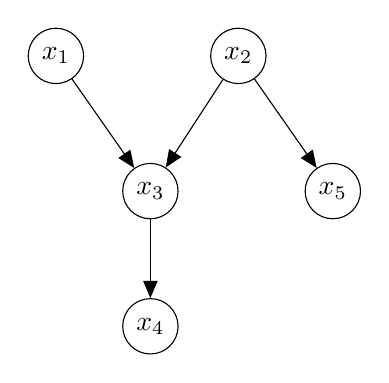
\begin{tikzpicture}[x=1.6cm,y=1cm]
        % Nodes
        \node[latent]               (x1) {$x_1$};
        \node[latent, right=of x1]  (x2) {$x_2$};
        
        \node[latent, below=of x1, xshift=1.2cm]  (x3) {$x_3$};
        \node[latent, right=of x3]  (x5) {$x_5$};

        \node[latent, below=of x3]  (x4) {$x_4$};

        \edge{x1, x2}   {x3}
        \edge{x3}       {x4}
        \edge{x2}       {x5}
    \end{tikzpicture}
    \caption{Simple DAG}
    \label{fig:dag1}
\end{figure}

A graph can be generated from a distribution and a (topological) ordering of the elements. A topological ordering is one where the parents come before the children. Note that different orderings may generate different graphs.

\subsection{Examples}

\textbf{Markov Models} (of order 1) or chains are a series of serial connections (\autoref{fig:markov}).

\begin{figure}[h]
    \centering
    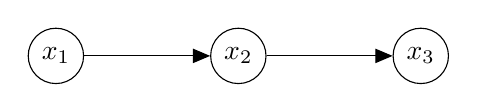
\begin{tikzpicture}[x=1.6cm,y=1cm]
        % Nodes
        \node[latent]               (x1) {$x_1$};
        \node[latent, right=of x1]  (x2) {$x_2$};
        \node[latent, right=of x2]  (x3) {$x_3$};
        
        \edge{x1}   {x2}
        \edge{x2}   {x3}
    \end{tikzpicture}
    \caption{Markov Chain}
    \label{fig:markov}
\end{figure}

\textbf{Hidden Markov Models} contain a markov chain that is not observed. Each hidden $\mathbf{h}$ influences an observable. $\mathbf{x}$'s are often at different timesteps, making the chain represent a time series. \autoref{fig:hidden_markov}.

\begin{figure}[h]
    \centering
    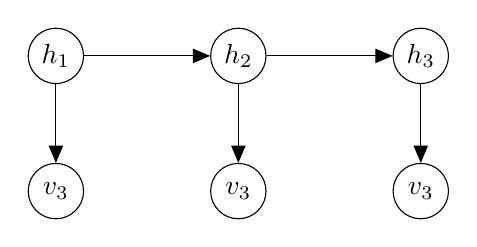
\begin{tikzpicture}[x=1.6cm,y=1cm]
        % Nodes
        \node[latent]               (h1) {$h_1$};
        \node[latent, right=of h1]  (h2) {$h_2$};
        \node[latent, right=of h2]  (h3) {$h_3$};
        \node[latent, below=of h1]  (v1) {$v_3$};
        \node[latent, below=of h2]  (v2) {$v_3$};
        \node[latent, below=of h3]  (v3) {$v_3$};
        
        \edge{h1}   {h2}
        \edge{h2}   {h3}
        \edge{h1}   {v1}
        \edge{h2}   {v2}
        \edge{h3}   {v3}
    \end{tikzpicture}
    \caption{Hidden Markov Model}
    \label{fig:hidden_markov}
\end{figure}

\textbf{Probabilistic PCA/ Independent Component Analysis} are methods that both use tha same graphical model. Here the latents (hiddens) variables are not connected. At the same time they influence all of the observables. \autoref{fig:ppca_lca}


\begin{figure}[h]
    \centering
    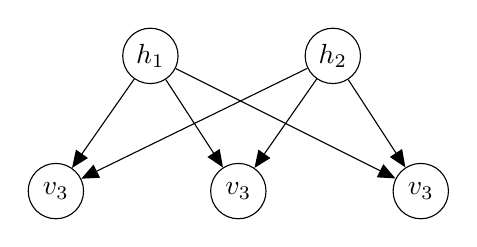
\begin{tikzpicture}[x=1.6cm,y=1cm]
        % Nodes
        \node[latent]               (h1) {$h_1$};
        \node[latent, right=of h1]  (h2) {$h_2$};
        \node[latent, below=of h1, xshift=-1.2cm]  (v1) {$v_3$};
        \node[latent, right=of v1]  (v2) {$v_3$};
        \node[latent, right=of v2]  (v3) {$v_3$};
        
        \edge{h1, h2}   {v1}
        \edge{h1, h2}   {v2}
        \edge{h1, h2}   {v3}
    \end{tikzpicture}
    \caption{PPCA/ ICA graphical model}
    \label{fig:ppca_lca}
\end{figure}

\subsection{D-Separation}
The main reason for using graphical models is to more easily determinite independencies between variables. In a DAG a tool for using this is D-separation. We start by examining the three possible trail connections in a DAG. Note that these are not all possible connections between three elements, but rather \textit{all possible connections when following a trail}.

\textbf{Serial Connections} are like Markov chains.

\begin{figure}[h]
    \centering
    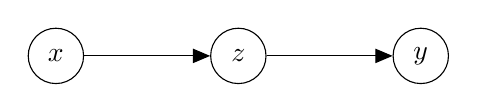
\begin{tikzpicture}[x=1.6cm,y=1cm]
        % Nodes
        \node[latent]               (x) {$x$};
        \node[latent, right=of x]   (z) {$z$};
        \node[latent, right=of z]   (y) {$y$};
        \edge{x}   {z}
        \edge{z}   {y}
    \end{tikzpicture}
    \caption{Serial Connecton}
    \label{fig:serial}
\end{figure}

Importantly we have:
\begin{gather*}
    \pr(x, z, y) = \pr(x) \pr(z \giv x) \pr(y \giv z) \\
    x \indep y \giv z \quad\quad x \notindep y
\end{gather*}

This means that if we know the variable $z$, x and y, \textbf{and all their parents and children} that are not connected to $z$ are independent of each other.

\textbf{Diverging Connections}
\begin{figure}[h]
    \centering
    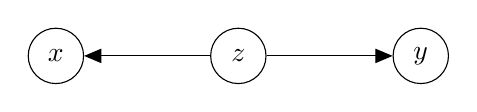
\begin{tikzpicture}[x=1.6cm,y=1cm]
        % Nodes
        \node[latent]               (x) {$x$};
        \node[latent, right=of x]   (z) {$z$};
        \node[latent, right=of z]   (y) {$y$};
        \edge{z}   {x}
        \edge{z}   {y}
    \end{tikzpicture}
    \caption{Diverging Connecton}
    \label{fig:divering}
\end{figure}

The same property of independence holds true here:
\begin{gather*}
    \pr(x, z, y) = \pr(z) \pr(x \giv z) \pr(y \giv z) \\
    x \indep y \giv z \quad\quad x \notindep y
\end{gather*}

\textbf{Converging Connections (Colliders)}
\begin{figure}[h!]
    \centering
    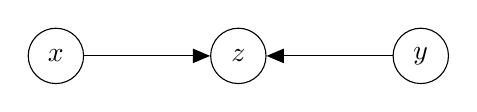
\begin{tikzpicture}[x=1.6cm,y=1cm]
        % Nodes
        \node[latent]               (x) {$x$};
        \node[latent, right=of x]   (z) {$z$};
        \node[latent, right=of z]   (y) {$y$};
        \edge{x}   {z}
        \edge{y}   {z}
    \end{tikzpicture}
    \caption{Collider}
    \label{fig:collider}
\end{figure}

For colliders if we \textbf{do not know $z$}, $x$ and $y$ are independent:
\begin{gather*}
    \pr(x, z, y) = \pr(z) \pr(x \giv z) \pr(y \giv z) \\
    x \indep y \quad\quad x \notindep y \giv z
\end{gather*}

This is true since $\pr(\cdot) = $...

\textbf{D-Separation}
Sets $X$ and $Y$ are d-separated by $Z$ iff all trails are blocked by $Z$. One of the following needs to be true for a trail to be blocked:

\textbf{1)} Either $b$ is in a head-tail or tail-tail configuration

\qquad
    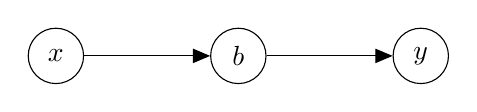
\begin{tikzpicture}[x=1.6cm,y=1cm]
        % Nodes
        \node[latent]               (x) {$x$};
        \node[latent, right=of x]   (b) {$b$};
        \node[latent, right=of b]   (y) {$y$};
        \edge{x}   {b}
        \edge{b}   {y}
    \end{tikzpicture} \qquad
    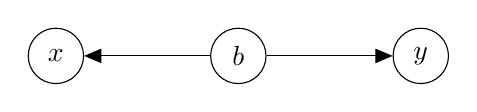
\begin{tikzpicture}[x=1.6cm,y=1cm]
        % Nodes
        \node[latent]               (x) {$x$};
        \node[latent, right=of x]   (b) {$b$};
        \node[latent, right=of b]   (y) {$y$};
        \edge{b}   {x}
        \edge{b}   {y}
    \end{tikzpicture}

and $b$ is in $Z$.

\textbf{2)} $b$ is a part of a collider

\qquad 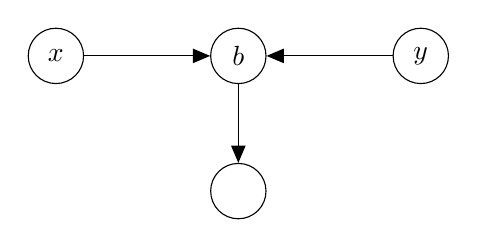
\begin{tikzpicture}[x=1.6cm,y=1cm]
    % Nodes
    \node[latent]               (x) {$x$};
    \node[latent, right=of x]   (b) {$b$};
    \node[latent, right=of b]   (y) {$y$};
    \node[latent, below=of b]   (e) {};
    \edge{x}   {b}
    \edge{y}   {b}
    \edge{b}   {e}
\end{tikzpicture}

and neither b or its descendents are in $z$. \textbf{Then} $X \indep Y \giv Z$.

\subsection{I-Maps}
A graph is an I-map for a set of independencies $I$ iff all independencies asserted by the graph are part of $I$. A graph can thus have fewer independencies than the set. A fully-connected graph is a trivial I-map for all sets $I$.

\subsection{Directed Local Markov Property}
\begin{equation*}
    \bx_i \indep (\pre \setminus \pa) \giv \pa \leftrightarrow \bx_i \indep (\text{nondesc}(\bx_i) \setminus \pa) \giv \pa
\end{equation*}

This [todo] figure.

\subsection{Gloabl directed Markov Property}
All independencies asserted by D-separation.

\subsection{Markov Blanket}
By definition:
$$
    x \indep (\text{all} \setminus \bx \setminus \text{MB}(\bx)) \giv \text{MB}(\bx)
$$
And for DAGs we get:
$$
    \text{MB}(\bx) = \text{pa}(\bx)\ \cup\ \text{children} (\bx) \ \cup\ \text{co-parents}(\bx)
$$

\section{Undirected Graphical Models}
Firstly, we note the following. For non-negative functions $a$ and $b$:

\begin{gather*}
    x \indep y \giv z \leftrightarrow \pr(x, y, z) = a(x, z) \times b(y, z) \\
    x \indep y \leftrightarrow \pr(x, y) = a(x) \times b(y) \\
    \sum_{x, y, z} a(x, z) b(y, z) = 1 \\
    \textbf{if} \   p(x, y, z) = \frac{1}{Z} \phi_A(x, z) \phi_B(y, z), \quad
    Z = \sum_{x, y, z} \phi_A(x, z) \phi_B(y, z)
\end{gather*}

\subsection{Gibbs Distribution}
.. is a distribution that factorizes as:
$$
    \pr(\bx) = \frac{1}{Z} \prod_c \phi_C(\mathcal{X}_C), \hspace{0.2in}
    \mathcal{X}_C \subseteq \{ x_1, \dots, x_d \}
$$

\subsection{Energy-Based Model}
If in the above $\phi_C(\mathcal{X}_C) = \text{exp} (- \text{E}_c(\mathcal{X}_c))$. Then:

$$
    \pr(\bx) = \frac{1}{Z} =
        \frac{1}{Z} exp \bigg[ - \sum_c \text{E}_c(\mathcal{X}_c) \bigg] =
        \frac{1}{Z} \prod_c \underbrace{\text{exp}^{
            -\text{E}_c(\mathcal{X}_c)
        }}_{\phi_c(\mathcal{X}_c)}
$$

\subsection{Undirected Graphs}
Assuming a distribution (up to a constant) factorizes as:

\begin{equation*}
    \pr(\bx) \propto \phi_1(x_1, x_2, x_3) \phi_2(x_2, x_3, x_4) \phi_3(x_3, x_5) \phi_4(x_5, x_6)
\end{equation*}

then we visualize it as the following graph:
\begin{figure}[h!]
    \centering
    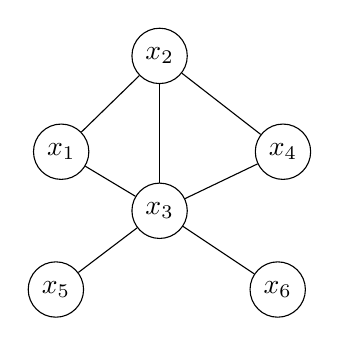
\begin{tikzpicture}[x=1.6cm,y=1cm]
        % Nodes
        \node[latent]               (x1) {$x_1$};
        \node[latent, right=of x1, xshift=.5cm]   (x4) {$x_4$};
        \node[latent, above=of x1, xshift=1.25cm, yshift=-.5cm]   (x2) {$x_2$};
        \node[latent, below=of x2, yshift=-.25cm]   (x3) {$x_3$};
        \node[latent, left=of x3, yshift=-1cm,xshift=1cm]   (x5) {$x_5$};
        \node[latent, right=of x5, xshift=.5cm]   (x6) {$x_6$};
        \edge[-]{x2, x3}   {x1}
        \edge[-]{x3, x4}   {x2}
        \edge[-]{x4, x5, x6}   {x3}
    \end{tikzpicture}
    \caption{Undirected Graph}
    \label{fig:ug}
\end{figure}

We form cliques for all variables in each factor $\phi_i$.

\subsection{Independencies in Undirected Models}
If
$$
    \pr(\bx) \propto \phi_1(x_1, x_2) \phi_2(x_2, x_3) \phi_3(x_4)
$$

Then the corresponding graph is:

\begin{center}
    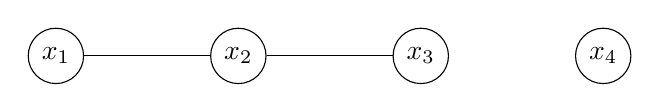
\begin{tikzpicture}[x=1.6cm,y=1cm]
        % Nodes
        \node[latent]               (x1) {$x_1$};
        \node[latent, right=of x1]  (x2) {$x_2$};
        \node[latent, right=of x2]  (x3) {$x_3$};
        \node[latent, right=of x3]  (x4) {$x_4$};
        \edge[-] {x1} {x2}
        \edge[-] {x2} {x3}
    \end{tikzpicture}
\end{center}

This directly implies that 
\begin{gather*}
    x_4 \indep x_1, x_2, x_3 \\
    x_1 \indep x_3 \giv x_2
\end{gather*}

In other words, a trail is blocked if there are no paths between the two nodes. Thus D-separation is more easily done here.

\subsection{Graph $\to$ Distribution}
Since we built undirected graphs by connecting cliques, it follows that given a graph we look at the maximum cliques to recover the distribution. \textbf{I-maps} are defined as before.

\subsection{Local Markov Property}
An edge is independent of all other edges given its neighbors. In the below graph the neighbors are colored in red. Formally, if $\text{ne}(\alpha)$ are the neighbors of $\alpha$, then:

$$
    \alpha \indep X \setminus (\alpha\ \cup\ \text{ne}(\alpha)) \giv \text{ne}(\alpha), \quad \forall \alpha \in X
$$


\definecolor{faintred}{RGB}{255,139,137}
\begin{center}
    \begin{tikzpicture}[x=1.6cm,y=1cm]
        % Nodes
        \node[latent]               (a) {$\alpha$};
        \node[latent, right=of a,fill=faintred]  (r) {};
        \node[latent, left=of a,fill=faintred]  (l) {};
        \node[latent, above=of a,fill=faintred]  (t) {};
        \node[latent, below=of a,fill=faintred]  (b) {};
        \node[latent, right=of r]  (r2) {};
        \node[latent, right=of t, xshift=0cm, yshift=1cm]  (t2) {};
        \node[latent, left=of b, xshift=.25cm, yshift=.25cm]  (bl) {};
        \node[latent, left=of l, yshift=.5cm]  (l2) {};
        \edge[-]{r, l, t, b} {a}
        \edge[-]{r2} {r}
        \edge[-]{t2} {t}
        \edge[-]{l, b} {bl}
        \edge[-]{l2} {l}
    \end{tikzpicture}
\end{center}

\subsection{Pairwise Markov Property}
\begin{equation*}
    \alpha \indep \beta \giv \underbrace{X}_{\text{all nodes}} \setminus \{ \alpha, \beta \}
\end{equation*}

for all non-neighboring $\alpha, \beta \in X$.


\definecolor{faintred}{RGB}{255,139,137}
\begin{center}
    \begin{tikzpicture}[x=1.6cm,y=1cm]
        % Nodes
        \node[latent]               (a) {$\alpha$};
        \node[latent, right=of a,fill=faintred]  (r) {};
        \node[latent, left=of a,fill=faintred]  (l) {};
        \node[latent, above=of a,fill=faintred]  (t) {};
        \node[latent, below=of a,fill=faintred]  (b) {};
        \node[latent, right=of r]  (r2) {$\beta$};
        \node[latent, right=of t, xshift=0cm, yshift=1cm,fill=faintred]  (t2) {};
        \node[latent, left=of b, xshift=.25cm, yshift=.25cm,fill=faintred]  (bl) {};
        \node[latent, left=of l, yshift=.5cm,fill=faintred]  (l2) {};
        \edge[-]{r, l, t, b} {a}
        \edge[-]{r2} {r}
        \edge[-]{t2} {t}
        \edge[-]{l, b} {bl}
        \edge[-]{l2} {l}
    \end{tikzpicture}
\end{center}

\subsection{Markov Blanket}
For undirected graph, the markov blanket of $x$ is the neighbors of $x$.

\noindent\fbox{%
    \parbox{\textwidth}{%
        N.B. All of the above properties (Markov properties) are equivalent for both directed and undirected graphical models. This means if one of them is true \textbf{for a distribution}, then all of them are true.
    }%
}

\textbf{TODO: Add Bishop plots with repetition boxes.}

\subsection{Minimal I-map}
\begin{itemize}
    \item[-] If an edge is removed, it ceases to be an imap.
    \item[-] A graph is an I-map if $\pr(\cdot)$ factorizes over the graph. 
\end{itemize}

\begin{varwidth}[t]{.5\textwidth}
    \textbf{Undirected Models}
    \begin{itemize}
        \item[-] For all $\bx_i$ find $MB(\bx_i)$ and connect.
    \end{itemize}
\end{varwidth}
\hspace{4em}
\begin{varwidth}[t]{.5\textwidth}
    \textbf{Directed Models}
    \begin{itemize}
        \item[-] For all $\bx_i$ find $\pi_i \subseteq \pre$ such that $\bx_i \indep \{ \pre \setminus \pi_i \} \giv \pi_i$
        \item[-] Set $\pa = \pi_i$
    \end{itemize}
\end{varwidth}

\section{Equivalence and Conversion Between Models}
Two directed graphs $G_1$ and $G_2$ are $I$-equivalent if they have the same set of immoralities and the same skeleton. An immorality is a collider without covering edge. \textbf{Look for colliders that don't match.} Since serial (head-tail) and diverging (tail-tail) connections imply the same independencies, we only need to look for converging (head-head) connections that don't match.

\subsection{Directed $\to$ Undirected}
We have:
\begin{equation*}
    \pr(\cdot) = \prod_i \pr(\bx_i \giv \pa) =
        \prod_i \underbrace{\phi_i(\bx_i, \pa)}_{\blue{cliques}}
\end{equation*}

\begin{itemize}
    \item[$\blacktriangleright$] This is called \textbf{moralization} and we obtain a \textbf{moral graph}
    % \item[$\vartriangleright$] This is called \textbf{moralization} and we obtain a \textbf{moral graph}
    \item[$\blacktriangleright$] This it \textbf{NOT} an undirected I-map for the distribution. Most notably
        we can not represent collider independencies. 
\end{itemize}

\subsection{Undirected $\to$ Directed}
(See example below)
\begin{itemize}
    \item[$\blacktriangleright$] Choose an ordering.
    \item[$\blacktriangleright$] Read independencies off of the graph and find $\pi_i$ for each $i$.
    \item[$\blacktriangleright$] Connect $\pi_i \to \bx_i$
\end{itemize}

\subsection{Non-equivalent Trails}
\textbf{Colliders can not be represented by undirected graphs.} 
\begin{center}
    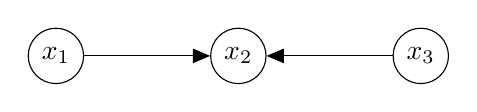
\begin{tikzpicture}[x=1.6cm,y=1cm]
        % Nodes
        \node[latent]               (x1) {$x_1$};
        \node[latent, right=of x1]  (x2) {$x_2$};
        \node[latent, right=of x2]  (x3) {$x_3$};
        \edge {x1} {x2}
        \edge {x3} {x2}
    \end{tikzpicture}
    \hspace{.5in}
    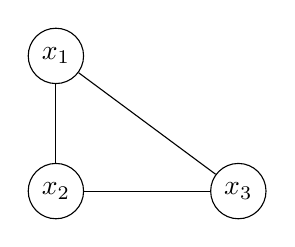
\begin{tikzpicture}[x=1.6cm,y=1cm]
        % Nodes
        \node[latent]               (x1) {$x_1$};
        \node[latent, below=of x1]  (x2) {$x_2$};
        \node[latent, right=of x2]  (x3) {$x_3$};
        \edge[-] {x1} {x2}
        \edge[-] {x3} {x2}
        \edge[-] {x1} {x3}
    \end{tikzpicture}
\end{center}
In the moralized graph on the
right the independence $\bx_1 \indep \bx_3$ is lost.

\textbf{Closed loops can not be represented by directed graphs.}
\begin{center}
    \begin{tikzpicture}[x=1.6cm,y=1cm]
        % Nodes
        \node[latent]               (x) {$x$};
        \node[latent, below=of x1, xshift=-1cm, yshift=.5cm]  (u) {$u$};
        \node[latent, below=of x1, xshift=1cm, yshift=.5cm]  (y) {$y$};
        \node[latent, below=of x1, yshift=-.5cm]  (z) {$z$};
        \edge[-] {u, y} {x}
        \edge[-] {u, y} {z}
    \end{tikzpicture}
    \hspace{.5in}
    \begin{tikzpicture}[x=1.6cm,y=1cm]
        % Nodes
        \node[latent]               (x) {$x$};
        \node[latent, below=of x1, xshift=-1cm, yshift=.5cm]  (u) {$u$};
        \node[latent, below=of x1, xshift=1cm, yshift=.5cm]  (y) {$y$};
        \node[latent, below=of x1, yshift=-.5cm]  (z) {$z$};
        \edge {x} {y}
        \edge {x, y} {u}
        \edge {u, y} {z}
    \end{tikzpicture}
\end{center} 

Consider the left graph. Let's review the process of creating the directed graph:
\begin{itemize}
    \item[$\blacktriangleright$] Choose an ordering: $x, y, u, z$.
    \item[$\blacktriangleright$] For each element, consider the parent set and read
        independencies off the directed graph.
    \item[$\blacktriangleright$] Start with $y \notindep x$, which implies the edge $x \to y$.
    \item[$\blacktriangleright$] Find the minimal set for which $u$ is independent of the parents $\pi_u$.
        This is $x, y$. Hence $x, y \to u$.
    \item[$\blacktriangleright$] For $z$ this set is $u, y$. Hence $u \to z$ and $y \to z$
\end{itemize}

\textbf{We no longer have the independence} $u \indep y \giv x, z$.

\section{Factor Graphs}
\begin{equation}
    \pr(\bx_1, \bx_2, \bx_3, \bx_4) = \frac{1}{Z} \phi_1(\bx_1, \bx_2, \bx_3)
        \phi_2(\bx_3, \bx_4) \phi_3(\bx_4)
\end{equation}

\begin{figure}[h]
    \centering
    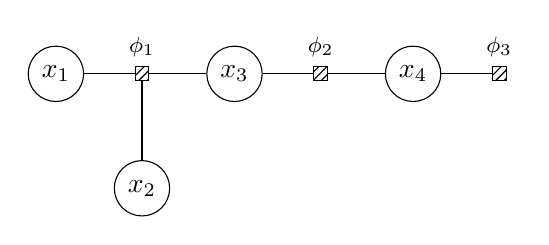
\begin{tikzpicture}[x=1.6cm,y=1cm]
        % Nodes
        \node[latent]               (x1) {$x_1$};
        \factor[right=of x1, pattern=north east lines, draw=black] {phi1} {$\phi_1$} {} {};
        \node[latent, below=of phi1]  (x2) {$x_2$};
        \node[latent, right=of phi1, xshift=-2.5em]  (x3) {$x_3$};
        \factor[right=of x3, pattern=north east lines, draw=black] {phi2} {$\phi_2$} {} {};
        \node[latent, right=of phi2, xshift=-2.5em]  (x4) {$x_4$};
        \factor[right=of x4, pattern=north east lines, draw=black] {phi3} {$\phi_3$} {} {};
        \edge[-] {x1, x2, x3} {phi1}
        \edge[-] {x3, x4} {phi2}
        \edge[-] {x4} {phi3}
    \end{tikzpicture}
    \caption{Factor Graph}
    \label{fig:factor_graph}
\end{figure}

\section{Exact Inference in Factor Graphs}
Assume discrete variables. The task is to compute $\pr(\bx_k = k)$ for all $k$.

We can group terms in the leaves of the tree. Consider:
\begin{equation}
    \pr(\cdot) \propto \phi_A(\bx_1) \phi_B(\bx_2) \phi_C(\bx_1, \bx_2, \bx_3)
        \phi_D(\bx_3, \bx_4) \phi_E(\bx_3, \bx_5) \phi_F(\bx_5)
\end{equation}

which is:
\begin{center}
    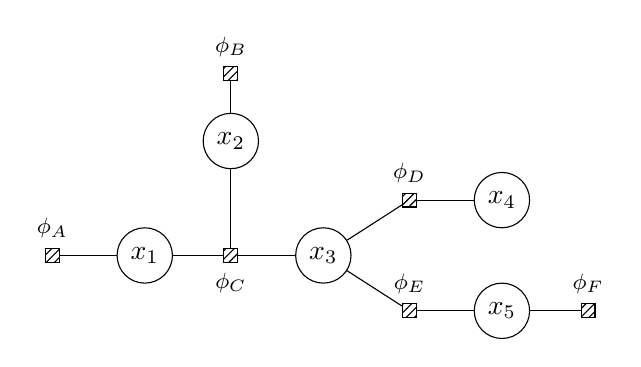
\begin{tikzpicture}[x=1.6cm,y=1cm]
        % Nodes
        \factor[pattern=north east lines, draw=black] {phia} {$\phi_A$} {} {};
        \node[latent, right=of phia, xshift=-2.5em] (x1) {$x_1$};
        \factor[right=of x1, pattern=north east lines, draw=black, label=below:$\phi_C$] {phic} {} {} {};
        \node[latent, right=of phic, xshift=-2.5em] (x3) {$x_3$};
        \node[latent, above=of phic] (x2) {$x_2$};
        \factor[above=of x2, pattern=north east lines, draw=black] {phib} {$\phi_B$} {} {};

        \factor[right=of x3, pattern=north east lines, draw=black, yshift=2em] {phid} {$\phi_D$} {} {};
        \factor[right=of x3, pattern=north east lines, draw=black, yshift=-2em] {phie} {$\phi_E$} {} {};

        \node[latent, right=of phid, xshift=-2.5em] (x4) {$x_4$};
        \node[latent, right=of phie, xshift=-2.5em] (x5) {$x_5$};
        \factor[right=of x5, pattern=north east lines, draw=black] {phif} {$\phi_F$} {} {};
        
        \edge[-] {x1} {phia}
        \edge[-] {x1, x2, x3} {phic}
        \edge[-] {x2} {phib}
        \edge[-] {x3, x4} {phid}
        \edge[-] {x3, x5} {phie}
        \edge[-] {x5} {phif}
    \end{tikzpicture}
\end{center}

We iteratively "eliminate" variables by summing or integrating them out. Firstly, we eliminate $\bx_5$:

\begin{align*}
    \pr(\bx_1, \dots, \bx_4) &= \sum_{\bx_5} \pr(\bx_1, \dots, \bx_5) \\
    &\propto \sum_{\bx_5} \phi_A(\bx_1) \phi_B(\bx_2) \phi_C(\bx_1, \bx_2, \bx_3)
    \phi_D(\bx_3, \bx_4) \phi_E(\bx_3, \bx_5) \phi_F(\bx_5) \\
    &\propto \phi_A(\bx_1) \phi_B(\bx_2) \phi_C(\bx_1, \bx_2, \bx_3)
    \phi_D(\bx_3, \bx_4) \sum_{\bx_5} \phi_E(\bx_3, \bx_5) \phi_F(\bx_5) \\
    &\propto \phi_A(\bx_1) \phi_B(\bx_2) \phi_C(\bx_1, \bx_2, \bx_3)
    \phi_D(\bx_3, \bx_4) \widetilde{\phi}_5(\bx_3)
\end{align*}

The idea is that we have reduced the factors above. Numerically, we would have the following:

\begin{equation*}
    \widetilde{\phi}_5(\bx_3) = \begin{cases}
        a \qquad \bx_3 = 1 \\
        \dots \\
        z \qquad \bx_3 = N \\
    \end{cases}
\end{equation*}

For each value of the factor. This is pre-computing all of the values, which in this case costs $O(N^2)$. For each value of $\bx_3$ we need to sum over $\bx_5$.

If we keep on doing this, the total cost will be greatly reduced from the $O(N^4)$ that is needed to sum over $\bx_2, \bx_3, \bx_4, \bx_5$.

The above operation is represented by the following \textbf{reduced} factor graph:

\begin{center}
    \begin{tikzpicture}[x=1.6cm,y=1cm]
        % Nodes
        \factor[pattern=north east lines, draw=black] {phia} {$\phi_A$} {} {};
        \node[latent, right=of phia, xshift=-2.5em] (x1) {$x_1$};
        \factor[right=of x1, pattern=north east lines, draw=black, label=below:$\phi_C$] {phic} {} {} {};
        \node[latent, right=of phic, xshift=-2.5em] (x3) {$x_3$};
        \node[latent, above=of phic] (x2) {$x_2$};
        \factor[above=of x2, pattern=north east lines, draw=black] {phib} {$\phi_B$} {} {};

        \factor[right=of x3, pattern=north east lines, draw=black, yshift=2em] {phid} {$\phi_D$} {} {};
        \factor[right=of x3, pattern=north east lines, draw=black, yshift=-2em] {phi5tilde} {$\widetilde{\phi}_5$} {} {};

        \node[latent, right=of phid, xshift=-2.5em] (x4) {$x_4$};
        
        \edge[-] {x1} {phia}
        \edge[-] {x1, x2, x3} {phic}
        \edge[-] {x2} {phib}
        \edge[-] {x3, x4} {phid}
        \edge[-] {x3} {phie}
    \end{tikzpicture}
\end{center}

\subsection{Message Passing}
\textbf{TODO: Graphs}
\begin{equation*}
    \mu_{\phi \to \bx}(\bx) = \sum_{\bx_1, \dots, \bx_j} \phi(\bx_1, \dots, \bx_j, x)
        \prod_{i = 1}^j \mu_{\bx_i \to \phi}(\bx_i)
\end{equation*}

\begin{equation*}
    \mu_{\bx \to \phi}(\bx) = \prod_{i = 1} ^ {j} \mu_{\phi_i \to \bx}
\end{equation*}

\begin{equation*}
    \prob(\bx) \propto \prod_{i = 1}^j \mu_{\phi_i \to \bx}(\bx)
\end{equation*}

\begin{equation*}
    \prob(\bx_1, \dots, \bx_j) \propto \phi(\bx_1, \dots, \bx_j)
        \prod_{i = 1}^{j} \mu_{\bx_i \to \phi} (\bx_i)
\end{equation*}

\section{Inference for Markov Chains}
\textbf{TODO: Just scan this..}
\subsection{$\alpha$-recursion}
\subsection{Smoothing}
\subsection{$\alpha$-$\beta$ Recursion}

\section{Model-Based Learning}
\begin{itemize}
    \item[--] Probabilistic model: table for a distribution $\prob(\bx)$
    \item[--] Statistical model: set of probabilistic models: $\{ \prob(\bx; \theta) \}$
    \item[--] Bayesian model: prior on theta, replace "parametrized by" with "conditioned on"
        $\prob(\bx) = \int \prob(\bx \giv \theta)\ \prob(\theta)$. To get the probability distribution
        of $\bx$ as above, we need to integrate over all possible values of $\theta$.
\end{itemize}

\section{Moment Matching}
Assume we have a parametric statistical model:

\begin{equation*}
    \prob(\bx; \theta) = \frac{
        \prob^*(\bx; \theta)
    } {
        Z(\theta)
    }
\end{equation*}

where $Z(\theta) = \int \prob^*(\bx; \theta)\ \text{d}\bx$ is the partition function. Maximum likelihood returns:

\begin{equation*}
    \theta^* = \argmax_\theta L(\theta) = 
        \argmax_\theta \sum_i \log \prob(\bx_i; \theta)
\end{equation*}

the last being true for i.i.d. data only. This directly implies that at the maximum, the derivative is $0$:

\begin{equation*}
    \nabla_\theta L(\theta) \vert_{\theta^*} = 0
\end{equation*}

We define the moments to be:
\begin{equation*}
    m(\bx; \theta) = \nabla_\theta \log \prob^*(\bx; \theta)
\end{equation*}

Then:

\begin{align*}
    \nabla_\theta L(\theta) &= \nabla_\theta \sum_i \log \prob(\bx_i; \theta) = \nabla_\theta \sum_i \log \frac{\prob^*(\bx_i; \theta)}{Z(\theta)} \\
    % 
    &= \bigg[\nabla_\theta \sum_i \log\prob^*(\bx_i; \theta) \bigg] - \nabla_\theta n \times \log Z(\theta) \\
    % 
    &= \sum_i \nabla_\theta \prob^*(\bx_i; \theta) - n \nabla_\theta \log Z(\theta) \\
    % 
    &= \sum_i m(\bx_i; \theta) - n \nabla_\theta \log Z(\theta)
\end{align*}

then for the second term we have:

\begin{align*}
    \nabla_\theta \log Z(\theta) &= \frac{1}{Z(\theta)} \nabla_\theta Z(\theta) = \frac{1}{Z(\theta)} \nabla_\theta \int \prob^*(\bx; \theta) \text{d} \bx = \\
    % 
    &= \frac{
        \int \nabla_\theta \prob^*(\bx; \theta) \text{d} \bx
    } {
        Z(\theta)
    } = \\
    % 
    &= \frac{
        \int \nabla_\theta \big[ \log \prob^*(\bx; \theta) \big] \prob^*(\bx; \theta) \text{d}\theta
    } {
        Z(\theta)
    } = \\
    % 
    &= \int \nabla_\theta \big[ \log \prob^*({\bx; \theta}) \big] \prob(\bx; \theta) \text{d}\bx \\
    % 
    &= \int m(\bx; \theta) \prob(\bx; \theta) \text{d}\bx
\end{align*}

which implies that:
\begin{equation*}
    \nabla_\theta L(\theta) = \sum_i m(\bx_i; \theta) - n \int m(\bx; \theta) \prob(\bx; \theta) \text{d} \theta
\end{equation*}

which means that at $\theta^*$, where $\nabla_\theta L(\theta) = 0$:
\begin{equation*}
    \frac{1}{n} \sum_i m(\bx_i; \theta) = \int m(\bx; \theta) \prob(\bx; \theta) \text{d} \theta
\end{equation*}

This proves that maximumum likelihood can be thought of as moment matching. We are matching the empirical moments to their expectation over the normalized data distribution $\prob(\bx; \theta)$. Note we don't have access to $\prob(\bx; \theta)$, but only to $\prob^*(\bx; \theta)$, the unnormalized distribution.

\section{Bayesian Inference}
This:
\begin{align*}
    \prob(\theta \giv \mathcal{D}) &= \frac{
        \prob(\theta; \mathcal{D})
    } {
        \prob(\mathcal{D})
    } = \frac{
        \prob(\mathcal{D} \giv \theta) \prob(\theta)
    } {
        \prob(\mathcal{D})
    } \\
    &\propto \text{Likelihood}(\theta) \prob(\theta) \propto \underbrace{\bigg[
        \prod_i \prob(\bx_i \giv \theta)
    \bigg]}_{\text{for i.i.d. data}} \prob(\theta)
\end{align*}

\section{Factor Analysis}
\begin{figure}
    \centering
    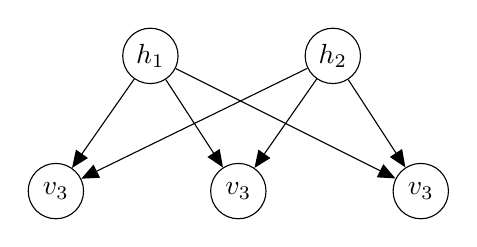
\begin{tikzpicture}[x=1.6cm,y=1cm]
        % Nodes
        \node[latent]               (h1) {$h_1$};
        \node[latent, right=of h1]  (h2) {$h_2$};
        \node[latent, below=of h1, xshift=-1.2cm]  (v1) {$v_3$};
        \node[latent, right=of v1]  (v2) {$v_3$};
        \node[latent, right=of v2]  (v3) {$v_3$};
        
        \edge{h1, h2}   {v1}
        \edge{h1, h2}   {v2}
        \edge{h1, h2}   {v3}
    \end{tikzpicture}
    \caption{FA/ICA graphical model}
    \label{fig:fa_ica}
\end{figure}

Both FA and ICA have the same (parametrized) graphical model. See \autoref{fig:fa_ica}. We have $D$ visible and $H$ hidden units:

$$
    \mathbf{h} \sim \mathcal{N}(\mathbf{0}, \mathbb{I}) \qquad H < D
$$
$$
    \prob(\mathbf{v} \giv \mathbf{\mathbf{h}}; \theta) = \mathcal{N}(\mathbf{v}; \mathbf{F} \mathbf{h} + \mathbf{c}, \psi)
$$

where:
$$
    \theta = \{ 
        \underbrace{\mathbf{c}}_{\text{mean of } \mathbf{x}},
        \mathbf{F} = 
            \underbrace{(f_1, \dots, f_H)}_{\text{factors of size D; F is DxH}},
        \Psi = 
            \underbrace{\text{diag}(\psi_1, \dots, \psi_D)}_{\text{noise variance}}
    \}
$$

This means that the model is:
\begin{align*}
    \mathbf{v} &= \mathbf{F} \mathbf{h} + \mathbf{c} + \mathbf{\epsilon} \qquad \epsilon \sim \mathcal{N}(0, \Psi)\\
    &= \sum_{i = 1}^H \mathbf{f}_i h_i + \mathbf{c} + \mathbf{\epsilon}
\end{align*}

\subsection{An important identity}
\begin{gather*}
    \text{if}\ \bx \sim \mathcal{N}(\mu_x, \mathbf{C}_x);
        \qquad \mathbf{z} \sim \mathcal{N} (\mu_z, \mathbf{C}_z) \\
    \mathbf{y} = \mathbf{A} \mathbf{x} + \mathbf{z},\
    \text{then} \qquad y \sim \mathcal{N}(
        \mathbf{A} \mu_x + \mu_z,
        \mathbf{A} \mathbf{C}_x \mathbf{A}^{T} + C_z
    )
\end{gather*}

\subsection{Factor Rotation Problem}
\begin{align*}
    \mathbf{v} &= \mathbf{F} \mathbf{h} + \mathbf{c} + \mathbf{\epsilon} = \mathbf{F} (\mathbf{R} \mathbf{R}^{T}) \mathbf{h} + \mathbf{c} + \mathbf{\epsilon} \\
    &= (\mathbf{F} \mathbf{R}) (\mathbf{R}^{T} \mathbf{h}) + \mathbf{c} + \mathbf{\epsilon} =
    (\mathbf{F} \mathbf{R}) \bar{\mathbf{h}} + \mathbf{c} + \mathbf{\epsilon}
\end{align*}

Which means that:
$$
    \prob(\bar{\mathbf{h}}) = \mathcal{N}(
        \bar{\mathbf{h}}; 0, \mathbb{I}
    )
$$
since $\mathbf{R}$ is an orthogonal matrix.

\section{Independent Component Analysis (ICA)}
ICA uses the same model as FCA but makes fewer assumptions. The joint of the hidden is:
% 
\begin{equation*}
    \prob_h(\mathbf{h}) = \prod_i p_h(h_i)
\end{equation*}
% 
with the observed (visible) following:
% 
\begin{equation*}
    \mathbf{v} = \mathbf{F} \mathbf{h} + \mathbf{c} + \epsilon 
\end{equation*}

\section{Intractable Likelihood Functions}
We'll look at three scenarios. Firstly, unobserved varibles. Assuming the following likelihood form:
% 
\begin{equation*}
    \text{L}(\theta) = \prob(\mathcal{D}; \theta) =
        \int_u p(\underbrace{\mathbf{u}}_\text{Unobserved}, \mathcal{D}; \theta)\ \text{d}\mathbf{u}
\end{equation*}
%
This is intractable, since we need to integrate over the observed, which are ... unobserved. We can use monte-carlo integration (below) if we know their distribution. However, it turns out that the gradient of the likelihood we can compute in a more convenient way:
% 
\begin{equation*}
    \nabla_\theta l(\theta) = \mathbb{E}_{\bu \sim \prob(\bu \giv \mathcal{D}; \theta)} \bigg[ \nabla_\theta \log \prob(\bu, \mathcal{D}; \theta) \giv \mathcal{D}; \theta \bigg]
\end{equation*}
% 
It is in most cases that we can compute the joint $p(\bu, \mathcal{D}; \theta)$ and conditional $p(\bu \giv \mathcal{D}; \theta)$. We can sample from the conditional and use Monte-Carlo integration.

TODO: proof

\subsection{Intractable Partition Function}
If the partition $Z(\theta)$ is intractable, we generally have the distribution up to a constant:
% 
\begin{equation*}
    \prob(\bx; \theta) = \frac{
        \prob^*(\bx; \theta)
    } {
        Z(\theta)
    }
\end{equation*}

Then we can use moment matching.

\begin{align*}
    \nabla_\theta l(\theta) &=  \sum_i m(\bx_i; \theta) - n \int m(\bx; \theta) \prob(\bx; \theta) \text{d} \theta \\
    &\propto \frac{1}{n} \sum_i m(\bx_i; \theta) - \mathbb{E} \big[ m(\bx; \theta) \big]
\end{align*}

where $m(\bx; \theta) = \nabla_\theta \prob^*(\bx; \theta)$

\section{Score Matching}
\section{Sampling and Monte Carlo}

\section{Sampling from Continuous Distributions}
\subsection{Rejection Sampling}
\subsection{Ancestral Sampling}
\subsection{Gibbs Sampling}

\section{Variational Inference}


% \printbibliography

\end{document}
